\documentclass{article}

\usepackage{graphicx}
\usepackage{tikz}
\usepackage{tikzsymbols}
\usetikzlibrary{calc,patterns,shapes.geometric}
\pagestyle{empty}
\usepackage[margin=0pt]{geometry}
\geometry{papersize={14in,12in}}

\def\centerarc[#1](#2)(#3:#4:#5){\draw[#1] ($(#2)+({#5*cos(#3)},{#5*sin(#3)})$) arc (#3:#4:#5);}

\begin{document}
	\begin{figure}
		\centering
		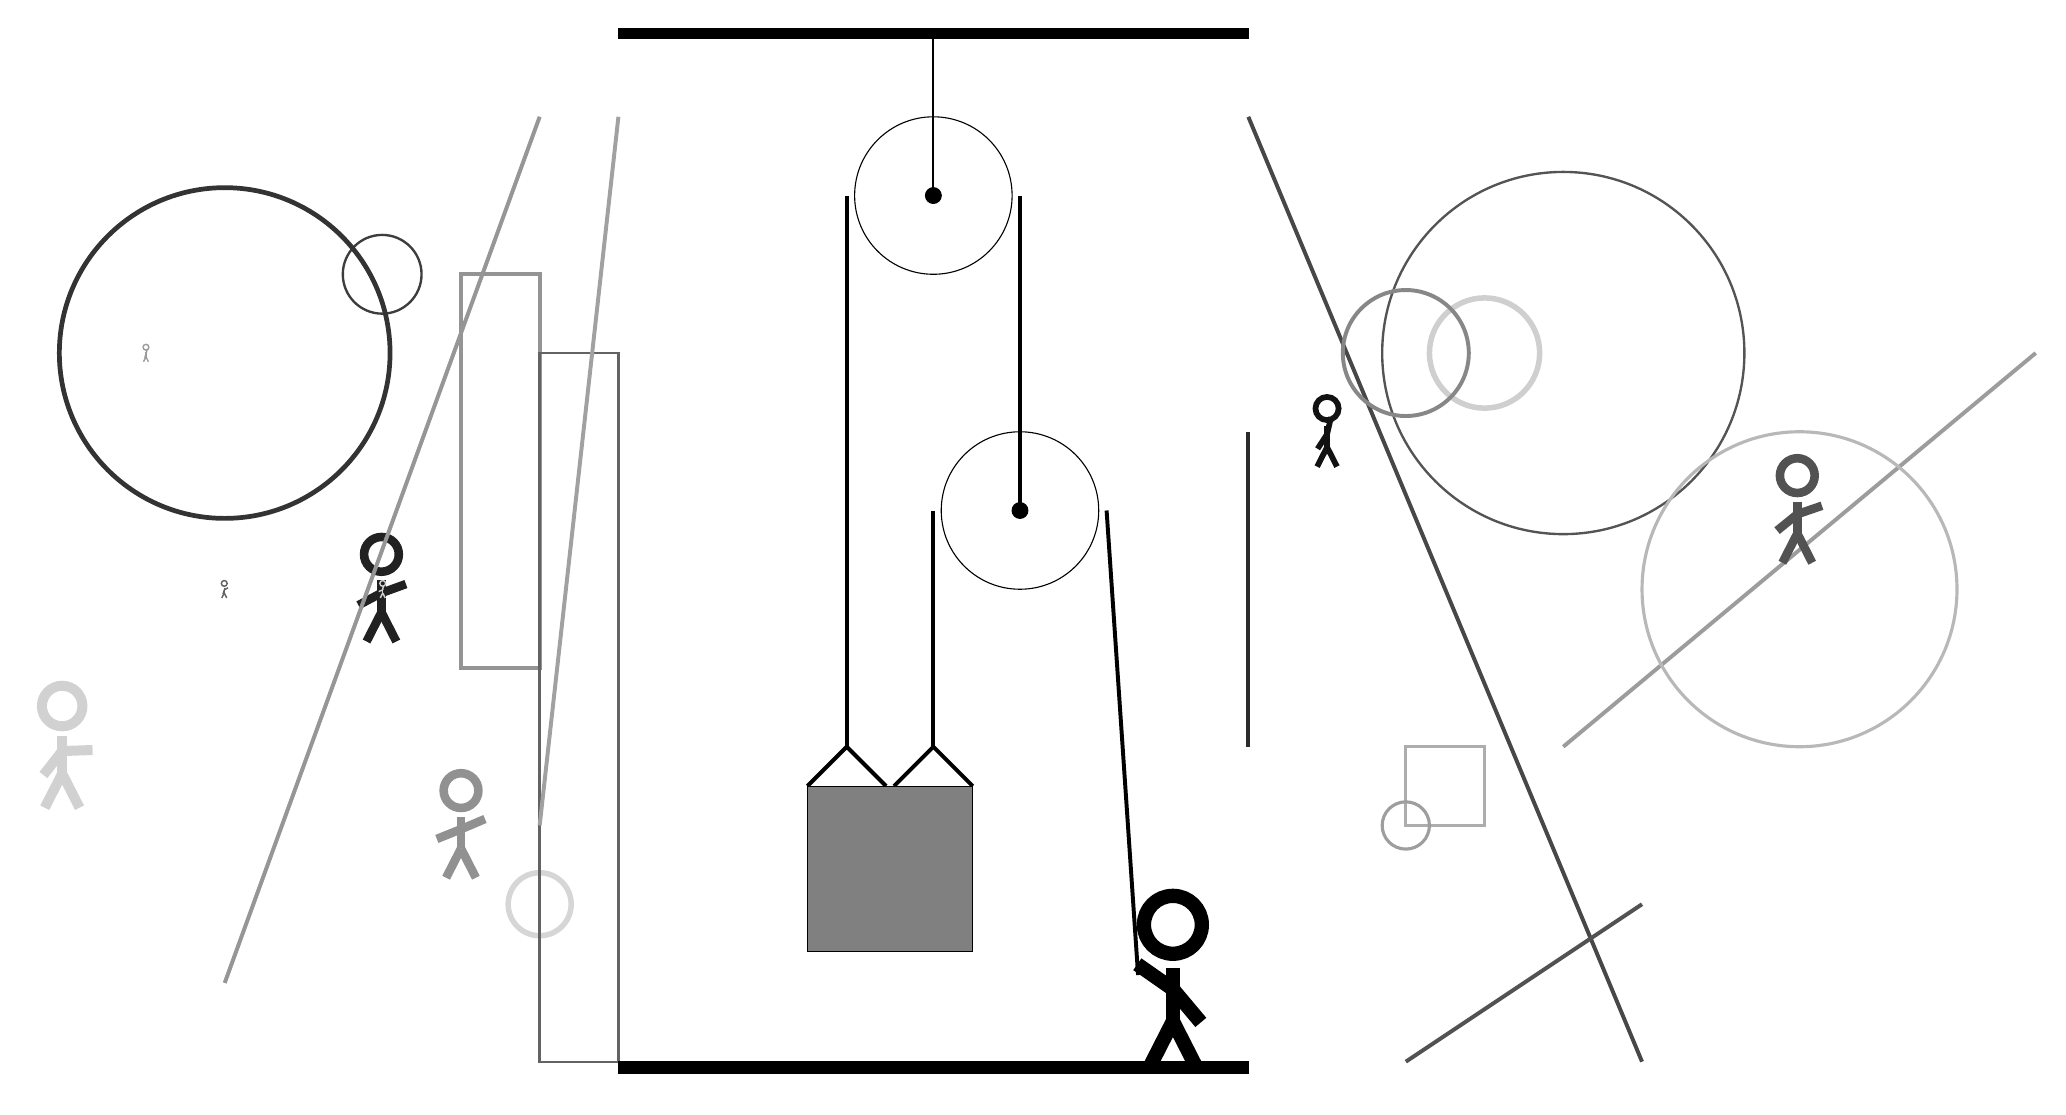
\begin{tikzpicture}
			%%%%% START %%%%%
			
			\draw[fill=black] (-2, 10) rectangle (6, 10.125);
			
			\draw (2, 8.0) circle (1);
			\draw[fill=black] (2, 8.0) circle (0.1);
			\draw[thick] (2, 8.0) -- (2, 10);
			
			\draw (3.1, 4.0) circle (1);
			\draw[fill=black] (3.1, 4.0) circle (0.1);
			
			\draw[line width = 0.5mm]  (0.4, 0.5) -- (0.9, 1.0) -- (1.4, 0.5);
			\draw[line width = 0.5mm]  (1.5, 0.5) -- (2.0, 1.0) -- (2.5, 0.5);
			\draw[fill=black!50] (0.4, 0.5) rectangle (2.5, -1.6);
			
			\draw [line width=0.7mm, color=black!16](-3, -1) circle (0.4);
			
			\node[line width=0.3mm, color=black!87] at (-5, 3) {\Strichmaxerl[6][28][20]};
			\draw[line width=0.5mm, color=black!42] (-4, 7) rectangle (-3, 2);
			\draw[line width=0.5mm, color=black!72](11, -3) -- (6, 9);
			\draw[line width=0.5mm, color=black!41](-7, -2) -- (-3, 9);
			\node[line width=0.4mm, color=black!39] at (-8, 6) {\Strichmaxerl[1][75][74]};
			\node[line width=0.5mm, color=black!18] at (-5, 3) {\Strichmaxerl[1][23][82]};
			\draw[line width=0.5mm, color=black!83](6, 1) -- (6, 5);
			\draw[line width=0.3mm, color=black!61] (-3, 6) rectangle (-2, -3);
			\node[line width=0.6mm, color=black!62] at (-7, 3) {\Strichmaxerl[1][74][29]};
			\node[line width=0.2mm, color=black!93] at (7, 5) {\Strichmaxerl[4][57][77]};
			\draw [line width=0.3mm, color=black!67](10, 6) circle (2.3);
			\draw [line width=0.3mm, color=black!76](-5, 7) circle (0.5);
			
			\draw [line width=0.7mm, color=black!19](9, 6) circle (0.7);
			\draw[line width=0.5mm, color=black!39](10, 1) -- (16, 6);
			\node[line width=0.4mm, color=black!18] at (-9, 1) {\Strichmaxerl[7][52][2]};
			
			\draw[line width=0.4mm, color=black!32] (8, 1) rectangle (9, 0);
			\draw [line width=0.4mm, color=black!38](8, 0) circle (0.3);
			\draw[line width=0.5mm, color=black!68](11, -1) -- (8, -3);
			\draw [line width=0.4mm, color=black!28](13, 3) circle (2.0);
			\node[line width=0.6mm, color=black!43] at (-4, 0) {\Strichmaxerl[6][22][23]};
			
			\draw [line width=0.5mm, color=black!47](8, 6) circle (0.8);
			\node[line width=0.6mm, color=black!68] at (13, 4) {\Strichmaxerl[6][39][19]};
			\draw [line width=0.6mm, color=black!80](-7, 6) circle (2.1);
			\draw[line width=0.5mm, color=black!37](-3, 0) -- (-2, 9);
			
			\draw[line width = 0.5mm] (0.9, 8.0) -- (0.9, 1.0);
			\centerarc[line width = 0.5mm](2, 8.0)(0:180:1.1);
			\draw[line width = 0.5mm] (3.1, 8.0) -- (3.1, 4.0);
			\draw[line width = 0.5mm] (2.0, 4.0) -- (2.0, 1.0);
			\centerarc[line width = 0.5mm](3.1, 4.0)(0:180:1.1);
			\draw[line width = 0.5mm] (4.2, 4.0) -- (4.6, -1.9);
			
			\node at (5, -2) {\Strichmaxerl[10][-35][-50]};
			
			\draw[fill=black] (-2, -3) rectangle (6, -3.15);
			
			%%%%% END %%%%%
		\end{tikzpicture}
	\end{figure}	
\end{document}